% !TEX root = ../thesis.tex

% Tässä osassa kuvataan käytetty tutkimusaineisto ja tutkimuksen metodologiset valinnat, sekä kerrotaan tutkimuksen toteutustapa ja käytetyt menetelmät.

% http://en.wikipedia.org/wiki/YUV#Y.27UV420p_.28and_Y.27V12_or_YV12.29_to_RGB888_conversion
% https://msdn.microsoft.com/en-us/library/windows/hardware/ff538197%28v=vs.85%29.aspx

% MITATTAVIA SUUREITA!

\documentclass[thesis.tex]{subfiles}

\begin{document}

\chapter{Design and Implementation}
\label{chapter:design-implementation}

\section{Requirements}

The goal was to implement a smartphone application that would satisfy the requirements listed below. Requirements \ref{R2} and \ref{R3} refer to the actual product authentication process, whereas requirements \ref{R1} and \ref{R4} are additional feature requirements:

\begin{enumerate}[leftmargin=0.55in, label=\textbf{R\arabic*}]
	\item \label{R1} Support the Windows Phone platform (preferably cross-platform)\\ \\
	Windows Phone was chosen as the target platform based on the Lumia 1020 smartphone, which was allocated for the project and featured one of the best smartphone cameras on the market (at the time). An additional goal was set for supporting other major platforms (Android and iOS) in the hopes of being able to compare the results across vendors.

    \item \label{R2} Capture the emission of a luminophore as a function of time\\ \\
    It was outlined that the application should be capable of capturing the emission as a sequence of images at a pre-defined interval that should not be longer than 1000ms. The sequence of captured images would work as a unique \emph{fingerprint}. Implementation details, such as the capture method (video vs. images), capture properties (e.g. ISO) or properties of the light source (e.g. wavelength, luminance) were not separately specified.
    % - in relation to Q1

    \item \label{R3} Use the capture data (fingerprint) to query a remote product database\\ \\
    The use case (product authentication) required that the fingerprint could be linked to a product. The requirement here was twofold: given a pre-defined database of fingerprints and products (1) characterize the capture data as a fingerprint and (2) match it against the existing fingerprints to find the linked product in remote product catalog.

	\item \label{R4} Support (secure) offline usage\\ \\
	Implementing support for offline usage was seen as an attractive feature that would differentiate the application from the competition. It would also allow investigating the feasibility of storing data client-side from a security and storage strategy perspective.
\end{enumerate}

\noindent The following chapters discuss these requirements further and present the related implementation details. Implementation for \ref{R1} and \ref{R2} is presented in Chapter \ref{chapter:application-architecture}. Requirements \ref{R3} and \ref{R4} are discussed in Chapters \ref{chapter:taggant-analysis} and \ref{chapter:storage-security}, respectively.

\section{Application Architecture}
\label{chapter:application-architecture}

The general architecture of the LuminoTrace application is depicted in Figure \ref{figure:architecture}. The camera application and the external camera module work in tandem to capture and analyze the taggant (luminophore) to construct a fingerprint. To find a product linked to the fingerprint a request is sent over the network to the application server, which queries the databases for a possible match. Alternatively, if the network is offline the application will fallback to querying a local, filtered copy of the database. Finally, the result of the search (match, no match or error) is renderer in the UI.

\begin{figure}[ht]
\centering 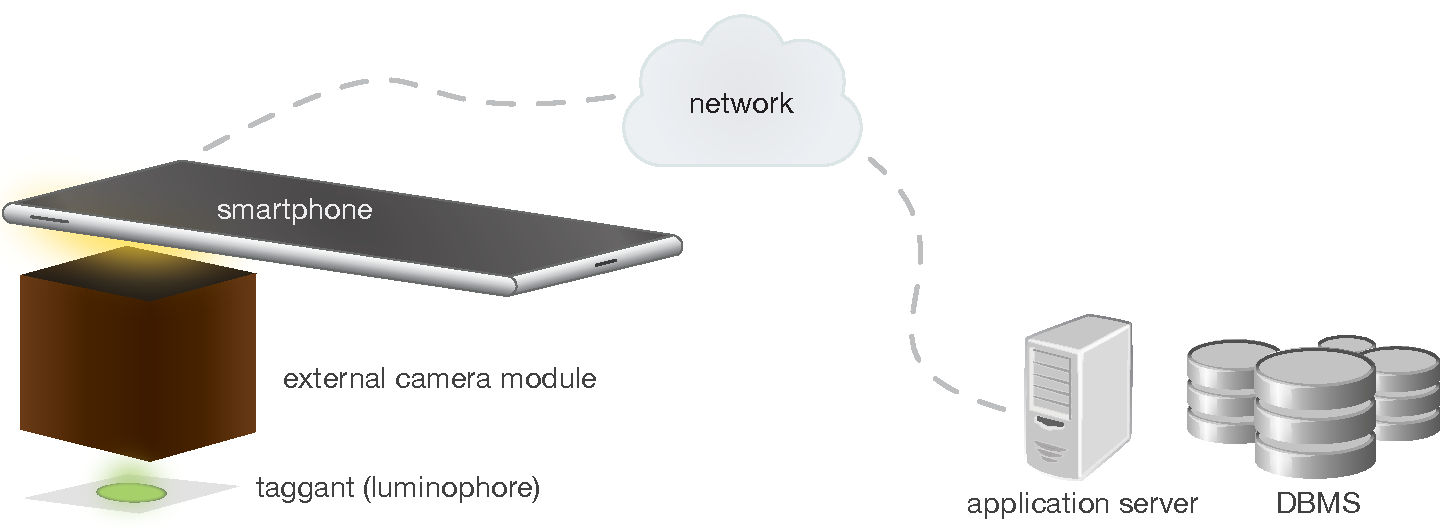
\includegraphics[width=13.5cm]{images/design_implementation/architecture}
\caption{An overview of the general architecture of the LuminoTrace application. \cite{inksure} \label{figure:architecture}}
\end{figure}

The next chapter will discuss the implementation of camera application in more detail. The other relevant parts of the architecture, namely the camera module, product authentication process

\subsection{Camera Application}
\label{chapter:camera-application}
ionic & cordova

error handling pages omitted for brevity

kuva vs. video

capture $->$ analyze $->$ match

- jni, c++/cx, ios with c++?
On iOS this extra bridge is unnecessary as C++ code can directly invoke Objective-C APIs.

kuva + kuva + kuva + kuva $=>$ fingerprint

\subsection{Camera Module}
ARDUINOOO
phosphorescence vs. fluorescence (infeasible coz time)

\section{Taggant Analysis}
\label{chapter:taggant-analysis}

\begin{comment}
\subsection{Color calibration}
\end{comment}
There are mainly two modules responsible for the color-rendering accuracy of a digital camera: the former is the illuminant estimation and correction module, and the latter is the color matrix transformation aimed to adapt the color response of the sensor to a standard color space. These two modules together form what may be called the color correction pipeline.

RGB is a device-dependent color model: different devices detect or reproduce a given RGB value differently, since the color elements (such as phosphors or dyes) and their response to the individual R, G, and B levels vary from manufacturer to manufacturer, or even in the same device over time. Thus an RGB value does not define the same color across devices without some kind of color management.

\url{http://www.cis.rit.edu/~jxj1770/publications/paperEI_Xerox.pdf}

\url{http://www.cs.unc.edu/techreports/04-012.pdf}

\subsection{Peak Finding}

\subsection{Similarity Matching}

\section{Storage and Security}
\label{chapter:storage-security}

The underlying server back end will consist of a web server and a database to hold the fingerprint data. Optionally, a reverse proxy can be set up in front of the web server to allow static assets to be served to the client without hitting the web server. However, since the application will most likely not include many static assets (images, JS, CSS...) the benefit of this is somewhat minimal. The back end will be implemented using Node.js due to its convenience (author's previous experience and the possibility to re-use the ported spectrum algorithm both in the front and back end). The database will be implemented with MongoDB as it couples well with Node.js and has cross-platform support and an active community.

Eventual consistency (CouchDB) (http://guide.couchdb.org/draft/consistency.html)
Schema flexibility

user management brute force

\end{document}